\chapter[Conclusions and Future Work]{Conclusions and Future Work}
\label{chap:Conclusions}

Research presented in this dissertation addresses the problem of how regular users can manage autonomy by managing information at different scale and hierarchy. This autonomy management approach is applied to the application domain of using a UAV to support Wilderness Search and Rescue. Autonomous components and autonomy management tools are designed at three distinctive scales, \textbf{Strategic}, \textbf{Between-Episodes}, and \textbf{Within-Episode}, following the autonomy integration guidelines we identified. And by managing two information representations, a \textit{probability distribution map} and a \textit{task-difficulty map}, at each scale, the domain expert user becomes an ``intelligent sensor'' and can feed information to each autonomous component in a form the autonomous component can understand. Doing so enables the user to influence the behavior of the autonomous subsystems without understanding the statistical models or complex algorithms used in the autonomous components.

%=====================================================================================================
\section{Conclusions}
\label{conclusions}

Challenges of integrating autonomy into an intelligent system can be characterized along two dimensions: \textit{attributes of an intelligent system} (capability, information management, performance evaluation) and \textit{scale} (individual, collaborative agents, distributed system). These attributes can serve as a guideline when designing autonomous components and autonomy management tools. We propose a new autonomy management approach where the user can influence the behavior of an autonomous system (or subsystem) by hierarchically managing information at different scales through two information representations:  a \textit{probability distribution map} and a \textit{task-difficulty map}. We designed autonomous components and autonomy management tools at each scale that enable the user to create and modify these maps by incorporating their domain knowledge and information. Then when these maps are used for UAV path planning, we developed multiple Intelligent Path Planning Algorithms that support real-time feedback and partial detection, and propose a sliding autonomy interface where the user can manage path planning autonomy by managing path segment endpoint constraints (spatial) and flight duration (temporal). We demonstrate the usefulness of this autonomy management approach and results from a user study show that this approach enables the human-automation team to outperform human or automation working alone, reduces the human's cognitive workload, and improves the human experience in the human-automation interaction.

%=====================================================================================================
\section{Contributions}
\label{contributions}

This dissertation has the following main contributions to Computer Science research.

\begin{itemize}
\item We identified autonomy integration challenges along two dimensions. These requirements served as a guideline in our design of the autonomous components and autonomy management tools in our proposed solution.
\item We propose a new autonomy management approach: managing autonomy by hierarchically managing information at three scales through two information representations: a \textit{probability distribution map} and a \textit{task-difficulty map}. We developed various autonomous components and autonomy management tools at each scale and demonstrated the usefulness of the approach.
\item We designed a Bayesian model that uses terrain features and past human behavior data to model lost-person behaviors. The user can influence the probability distribution map generated by changing prior beliefs and by selecting what subset of past human behavior data to feed to the model.
\item We designed two autonomy management tools that enable the user to manage the \textit{probability distribution map} and \textit{task-difficulty map} by mouse and finger gestures.
\item We proposed a heuristic, \textit{Mode Goodness Ratio}, which uses a Gaussian Mixture Model to prioritize search subregions, and enables a hierarchically search for effective paths through the parameter space at different levels of resolution.
\item We designed multiple path planning algorithms that support partial detection. We evaluated the performance of these algorithms against state-of-the-art algorithms using three real WiSAR scenarios and show that our algorithms generate near-optimal paths in real-time.
\item We proposed the Sliding Autonomy Interface that enables the user to manage path planning autonomy along two dimensions: constraints (spatial) and flight duration (temporal). Data from a user study show that this approach enables the human-automation team to outperform human or automation working alone, reduces the human's cognitive workload, and improves the human experience in the human-automation interaction.
\end{itemize}

%=====================================================================================================
\section{Future Work}
\label{futurework}

This section presents a few of the natural extensions from current research that can be pursued as future work. We list them in the order of the three scales and show how they relate to the various components of the dissertation work (see Figure~\ref{ProjectComponents2}).

\begin{figure}
\centering
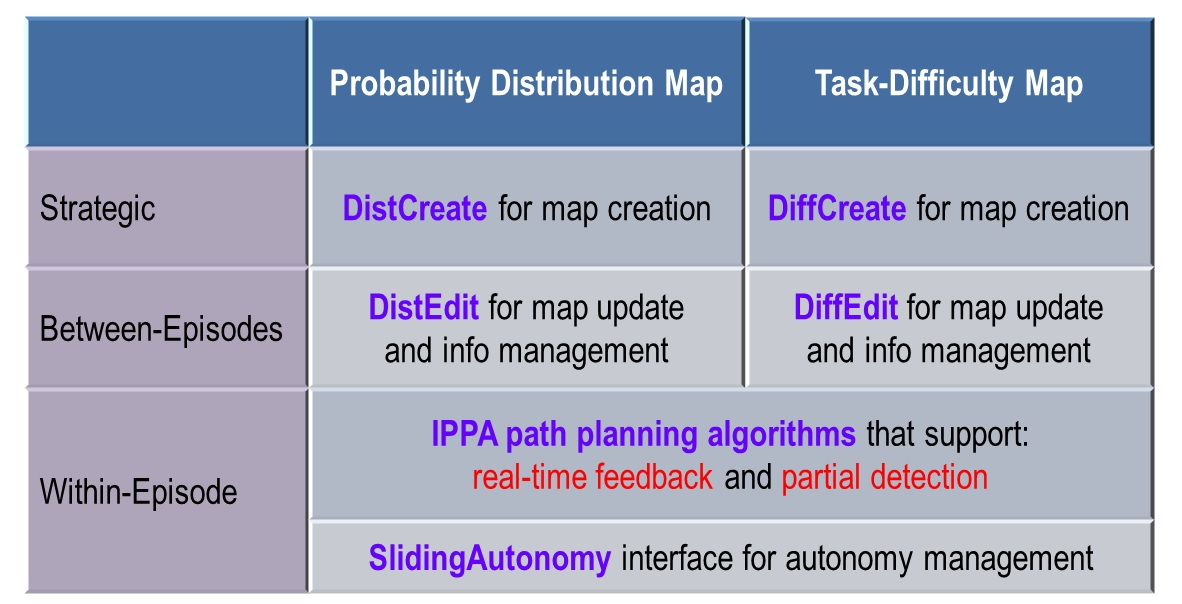
\includegraphics[width=6in]{ProjectComponents.JPG}
\caption{Autonomous components and autonomy management tools of the dissertation work at each scale/hierarchy.}
\label{ProjectComponents2}
\end{figure}

%===================================================
\subsection{At the Strategic Scale}

Presently the \textbf{DistCreate} component uses a set of default prior belief parameters (transitional probabilities between pairs of terrain features) which can be changed by the domain expert user based on his her her domain expertise and information only the user can interpret. It would be beneficial if the system can automatically suggest transitional probability values based on statistics from past incidents~\cite{Koester2008Lost} after the user provides some initial lost person profile information (such as age, gender, etc.). When the user wants to modify the suggested parameters, instead of typing in values, it would be helpful to provide a tool that allows the user to visually see the prior belief distributions. By moving two sliders to change the mean and standard deviation values, the user can actually see how the shapes of the distributions changes. Ideally, the user can also see how this affects the shapes of the final prior / posterior predictive probability distributions with instant feedback. This immediate visual feedback allows the user to understand causal effects and therefore helps the user form a mental model of the system that is similar to how the system truly works. Figure~\ref{Mockup1} shows a mock up screen of such a tool. Computationally, instant feedback would require that we perform complex matrix computations on the GPU using CUDA (Compute Unified Device Architecture) architecture. Then to evaluate how this affects the human-automation interaction and the performance of the human-automation team, a user study can be performed.

\begin{figure}
\centering
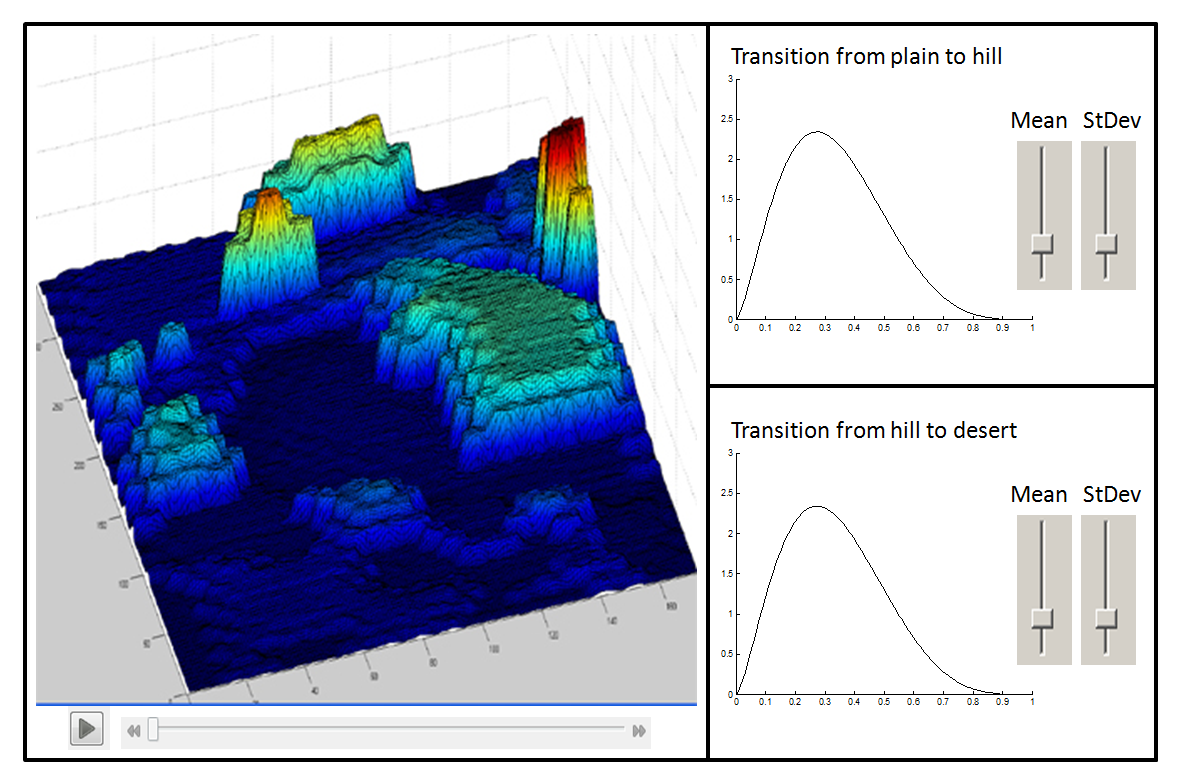
\includegraphics[width=6in]{Mockup1.png}
\caption{A mock up screen for the management tool interface at the general trend scale.}
\label{Mockup1}
\end{figure}

The \textbf{DistCreate} component considers three terrain features: topography, elevation, and vegetation density. It is probably beneficial to incorporate more factors that affect lost-person behaviors into the network. Such factors include but are not limited to direction of travel, trail following, missing person profile, panicking factor, weather conditions and season of the year. Such factors can be easily included into the existing Bayesian network as prior nodes. Additional utility tools might be needed to generate geographic data when it is not directly available. For example, if trail data cannot be automatically extrapolated, such utility tools would allow the search to manually mark trails on a map.

Currently the user can only specify whether to use past-human behavior data or not with the \textbf{DistCreate} component. In the future, as more past-human behavior data become available, the data can be stored in a database, and the user can further decide which subset of the behavior data to use by querying the database. For example, the user can choose to only use data of the same search region, season of the year, or data matching the missing person profile.

The \textbf{DiffCreate} component uses vegetation coverage data from USGS satellite imagery data to extrapolate vegetation density and determines task difficulty (detection probably). This is a very simple model that is included in our dissertation for completeness and demonstration purposes. A more advanced model can be designed to include additional factors such as UAV height above ground, time of the day, season of the year, ``seeability''~\cite{Morse2010UAV}, sensor specific properties (e.g., an infrared multi-spectrum camera). Additional constraints such as no-fly zone or dangerous areas can also be included in the \textit{task-difficulty map}.

%===================================================
\subsection{At the Between-Episodes Scale}

The \textbf{DistEdit} and \textbf{DiffEdit} components at this scale let the user use mouse and finger gestures to edit the \textit{probability distribution map} and the \textit{task-difficulty map} generated from the higher scale in a 3D environment. In this dissertation we only validated the usefulness of these two tools by demonstration. To better evaluate the usefulness of the two tools, a well-designed user study should be performed. Ideally, these tools should be given to real search and rescuers to generate maps for real WiSAR scenarios. The user should be able to modify these maps as new information becomes available. For example, when a piece of clothing or candy wrap is found during the search, or when ground searchers have thoroughly searched an area and confirmed that the missing person is unlikely located at certain regions. These tools can also be integrated with the Sliding Autonomy component in the next scale so the two maps can be updated in real time while the UAV is in the air during the mission.

%===================================================
\subsection{At the Within-Episode Scale}

At this scale we designed multiple Intelligent Path Planning Algorithms that supports real-time feedback and partial detection. Although these algorithms assume the missing person is stationary and the probability distribution map and the task-difficulty map are static, because these algorithms are very fast, it should be possible to improve the algorithms to deal with moving targets, changing probability distribution and a task-difficulty map that changes over time. Then to further expand the problem, these algorithms can be improved to work with multiple targets or support multiple UAVs. We leave these to future work.

The \textbf{SlidingAutonomy} interface allows the user to work with automation as a team and affect the behavior of the path planning autonomy by setting constraints and play with different flight duration. The user study we performed is a short-term study where each user only had a short training before using this interface. Because human's trust in autonomy can change over time, it would be interesting to research how the user's trust gets calibrated when the user uses this autonomy management approach for a long period of time. Would the user be able to gradually identify the weaknesses of the path planning autonomy and remedy correctly? Would the user overtrust autonomy and perform worse in the long run? Or would the user undertrust autonomy because autonomy makes obvious mistakes in certain scenarios? These questions can only be answered with a long-term user study, which we leave for future work.

At this scale, while the UAV is in the air during mission, as information is collected and processed by the collective search and rescue team, situation arises when the \textit{probability distribution map} and/or the \textit{task-difficulty map} become incorrect. In cases where these two maps cannot be updated in real-time, how can the user use \textbf{SlidingAutonomy} to manage UAV path planning autonomy to address the information change, maybe avoid certain regions or force the UAV to visit certain regions repeatedly, is another interesting research topic. A user study can be performed to evaluate the human-automation interaction experience and the performance of this Sliding Autonomy approach.


%===================================================
\subsection{The Overall Autonomy Management Approach}

In this dissertation we applied the proposed autonomy management approach to the application domain of using a UAV to support Wilderness Search and Rescue. It is worth mentioning that this approach can be generalized and applied to many application domains. For example, when using an assistive robot to help a therapist treat children with autism, robot autonomy can also be managed by hierarchically managing information at different scales. 

At the \textbf{Strategic} scale, before an autistic child begins clinical treatments, the therapist performs a series of evaluations. Information collected is analyzed to determine the deficiencies, then a treatment plan is created identifying areas the therapist should focus on (e.g., joint attention, turn taking). Here this areas of focus map is equivalent to the \textit{probability distribution map} we discussed before. It is possible to develop a model to assist the therapist in generating this initial plan at the general trend scale. The therapist can decide what model parameters and dataset to use to train the model or to affect the plan. Similarly, a \textit{task-difficulty map} can be created identifying areas where the therapy treatment might not be very effective.

At the \textbf{Between-Episodes} scale, typically an autistic child receives one or two treatments each week. At different stages of the treatment the therapist might focus on different areas or reinforce certain behaviors in each session. The therapist may prefer the robot to have exaggerated facial expression and movement in one session but appear calmer and more verbose in another; or the therapist might want the robot to demonstrate a higher degree of reliance on the therapist some times. Ideally, by adjusting the areas of focus and the task-difficulty map at the between-sessions scale, the therapist can take advantage of special knowledge or experience and indirectly affect the robot's autonomous behaviors by managing what information to provide.

At the \textbf{Within-Episodes} scale, during a clinical session an autistic child might not behave as the therapist expects (due to fatigue, previous events, or unexpected events). The therapist needs to be able to manage the robot's autonomous behaviors in real-time in order to improve or maximize the potentials of the treatment. The ability to modify the areas of focus and the task-difficulty map in real time affords the therapist the desired levels of control. The therapist can also strategically plan out the order of activities (targeted to different deficiencies) and desired intensity (time allocated to each activity) during the session to improve the efficiency of the treatment. At the within-session scale, the therapist is really actively collecting information (the child's behavior and reaction), digesting the information, and then decide what information to provide to the system, in forms the system can understand, in order to manage the autonomous behavior of the robot.

Applying our proposed autonomy management approach to a completely different application domain and then evaluate how well the approach generalized is an important part of future work.